\chapter{Evaluation and Discussion}
\label{chap:eval}

% пошутить про kisp и мейера

In this chapter we are going to present our approach to the testing and evaluation of the three main components: KISP
Interpreter, Visualiser and Virtual Assistant. Among many other types of software assessment, we chose the following methods
due to their effectiveness and relative simplicity: Benchmarking, Conditional and Unit Testing.

\section{Conditional Testing}
In the field of Computer Science the idea of \textit{design by contract} is well-known: programmer uses pre- or post-conditional
statements to control the source code execution. There are many languages with native support of these features, including
Eiffel\cite{eiffel}, created by Bertrand Meyer. In Java we can use the keyword \texttt{assert} to simulate their behaviour.
What makes Java assertions special is that we can turn them on and off manually by supplying the
\texttt{-enableassertions} key to the JVM's argument list, thus removing their computational overhead.

During the coding phase, we wrote $93$ assertion statements that mainly control the execution of KISP interpreter.
Then we manually tested the application to see whether any of them would fail, but none ever did.

\section{Unit Testing}
This type of software testing is ubiquitous in the industry, especially in the \textit{Test-Driven Development} process, where
requirements are turn into test cases, and then the software is improved to pass these tests only.
Historically, the idea of TDD was firstly used in the \textit{Extreme Programming} methodology, invented\cite{beck} by
engineer Kent Beck in 1999.

There are many solutions for the Java language that implement the concept of Unit Testing. Among many others, we decided to use
JUnit\cite{junit} $5$ library, which was also developed by Kent Beck et al., to write $136$ test cases that cover $100$\% of KISP
classes, $81,3$\% of interpreter's methods and $79,7$\% of its lines. Using this library, we have tested all standard KISP
functions and types, only to ascertain that everything works as intended and all tests pass.

\section{Interpreter Benchmarking}
One of our main goals was to achieve an adequate performance of the KISP interpreter. In order to ascertain whether we attained
that goal or not, we ran a benchmark test and collected its results. We chose the implementation of the \texttt{factorial}
function as the benchmark target, and ran it of $40$ different inputs.
\begin{verbatim}
(define factorial
    (lambda (n) (if (= n 0) 1 (* n (factorial (dec n))))))
\end{verbatim}

From the results of the first benchmarking session \ref{fig:bench1}, we can see how our \textit{caching} mechanism affects the
performance of the factorial procedure: if at the beginning the execution time have risen to almost $4$ milliseconds,
subsequent runs demonstrate significant improvements, ending in being just below a millisecond.
In the second session \ref{fig:bench1}, we supplied larger values of $N$, but as we can see, we got a similar picture, only the
initial discrepancy is larger this time.

These two benchmarking sessions clearly show that we indeed reached our third goal. The performance of KISP interpreter is withing
the expected norms, thanks to the caching mechanism. However, it can be significantly improved further by introducing
\textit{Just-in-Time} compilation.
\begin{figure}[h!]
    \centering
    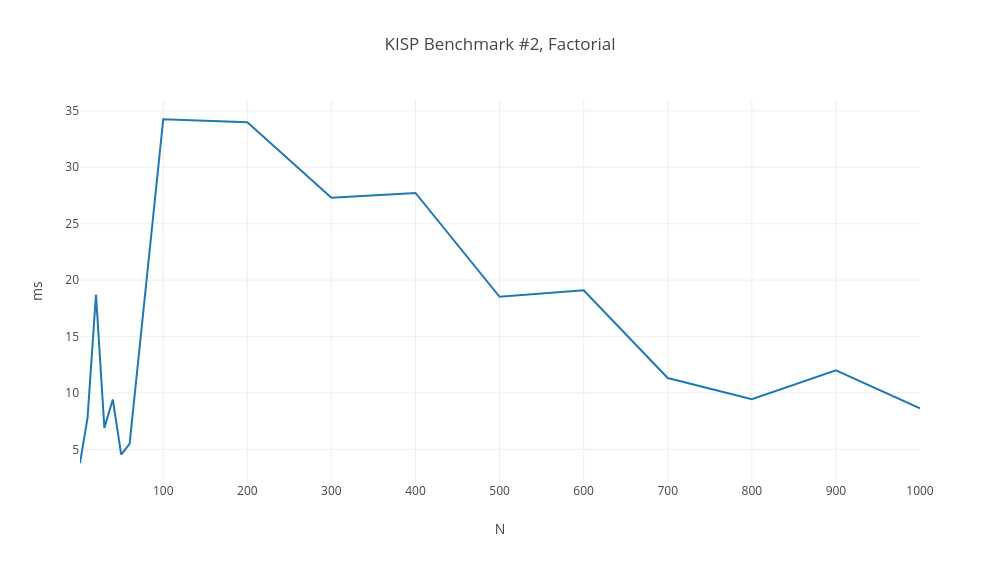
\includegraphics[width=\linewidth]{figs/kisp-bench2.png}
    \caption{Second Benchmarking Session}
    \label{fig:bench2}
\end{figure}
\begin{figure}[h!]
    \centering
    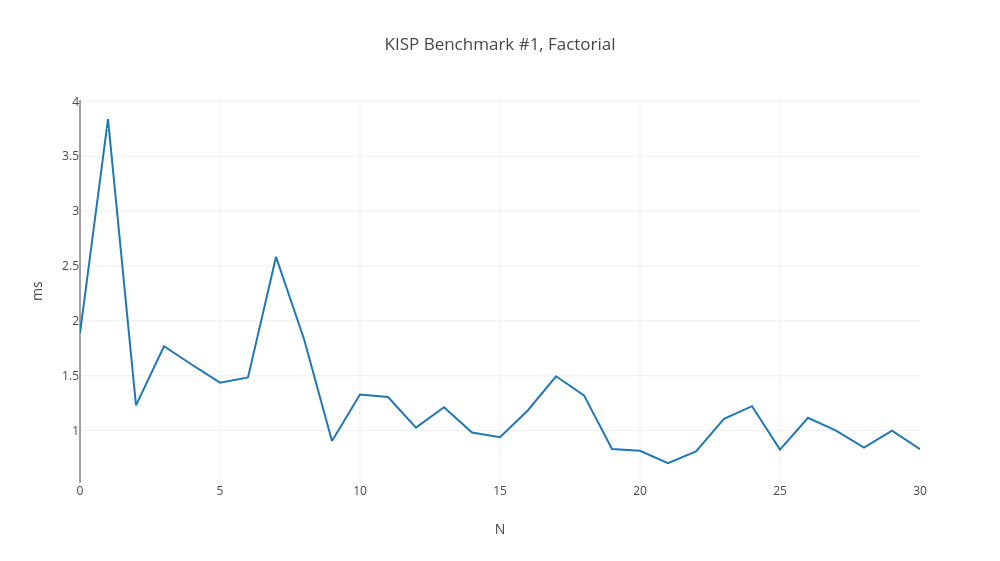
\includegraphics[width=\linewidth]{figs/kisp-bench1.png}
    \caption{First Benchmarking Session}
    \label{fig:bench1}
\end{figure}
